\section{Proposal}
\label{proposal}

\subsection{Analysis of Web Service documentation sources}
\label{subsec:analysis-ws-doc}
As evidenced in the study by Maleshkova et al. \cite{Maleshkova:2010}, web service documentation is often limited by the content that API developers provide on their websites. SOAP services are a special case, whose main descriptor is a WSDL document, which defines an abstract service interface (information regarding operations, messages and types) and concrete details about transport and location of the service. Following subsections deal with the description of mechanisms for extraction of technical information regarding service functionality, from various documentation sources: WSDL descriptors for SOAP services, and HTML pages for XML-RPC and REST services.

\subsubsection{SOAP Services}
\label{subsubsec:soap}
WSDL is an XML standard format for Web service description [32]. A WSDL document describes service interface abstractly and provides concrete technical details about service operation. This may be visualized in figure \ref{wsdl-Structure}, which shows the structure of a WSDL descriptor.

\begin{figure}
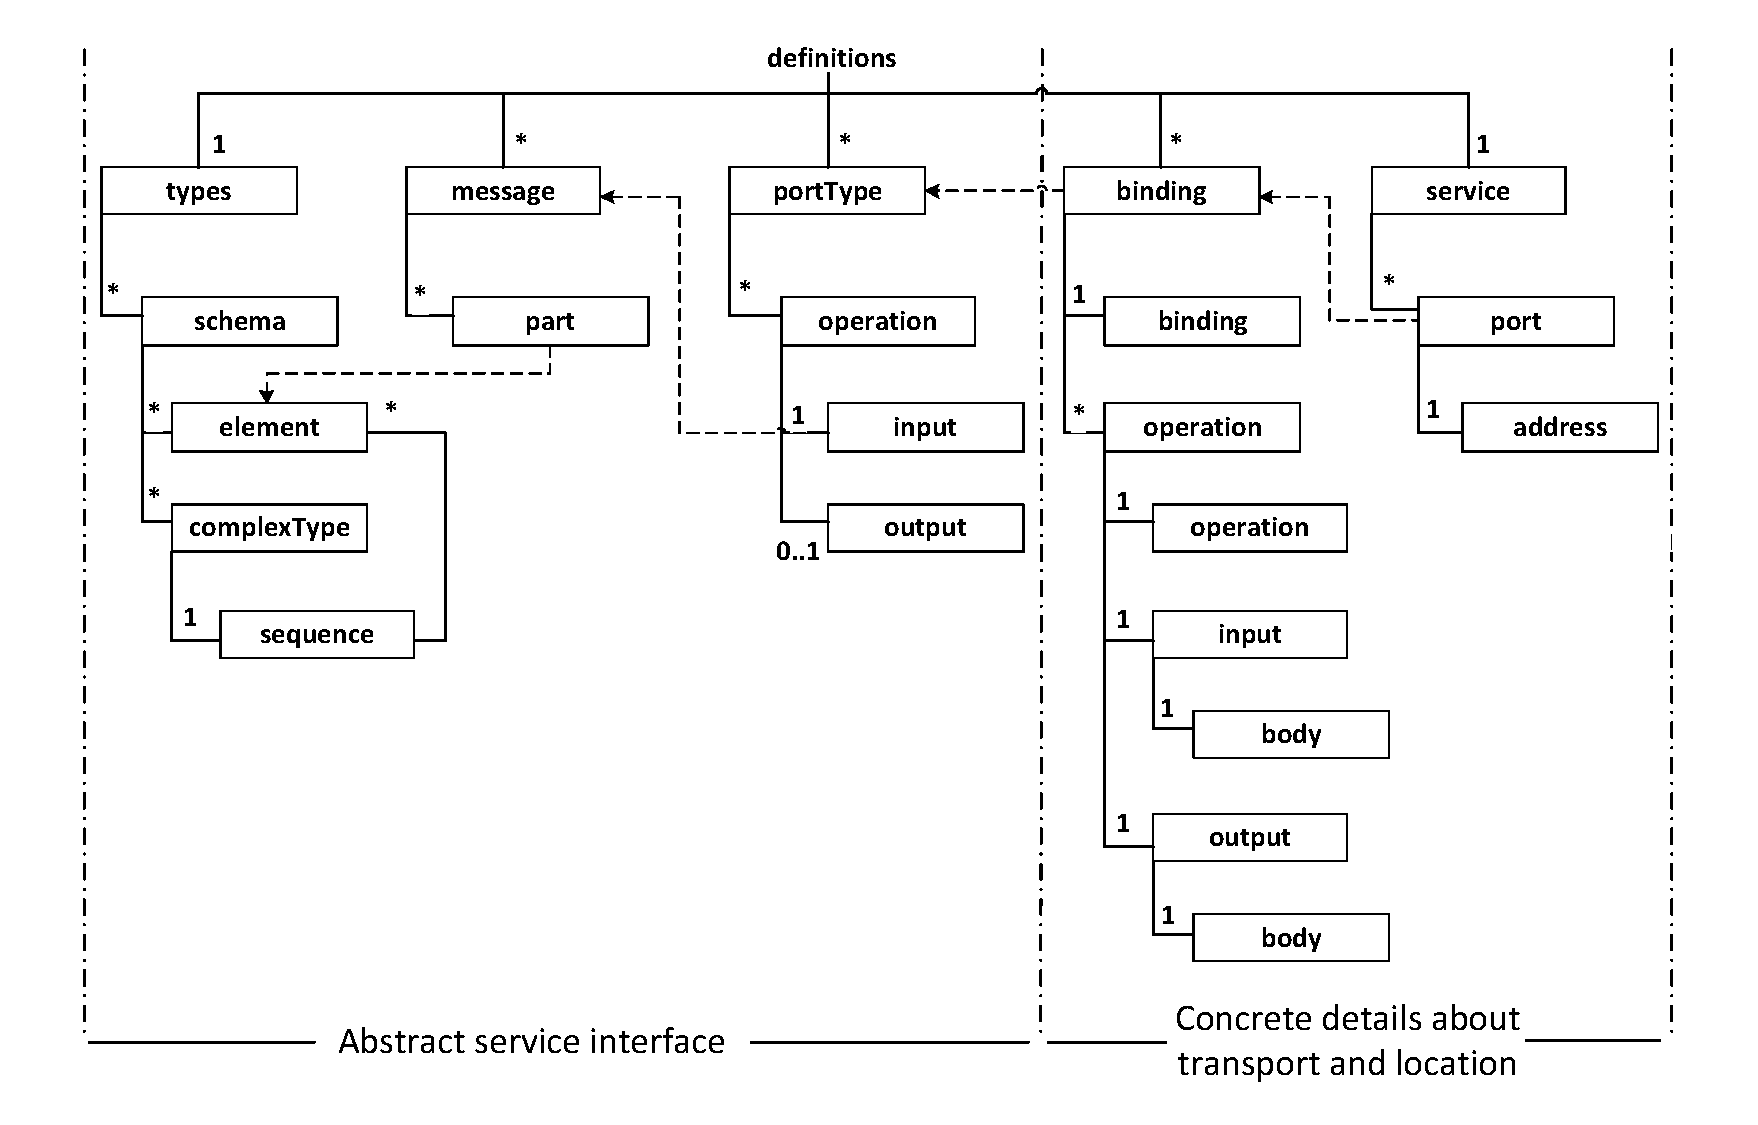
\includegraphics[scale=0.40]{images/wsdl-structure-en}

\caption{Structure of WSDL descriptor.}
\label{wsdl-Structure}
\end{figure}

The diagram of figure \ref{wsdl-Structure}, shows the separation between service’s abstract description and concrete details. The later refer to element that specify service endpoints, and communication and transport protocols used for message exchange. These concrete details are required for service invocation, however they provide little information about service functionality, this is why descriptor analysis focuses on the components of the abstract description of the service interface, namely:

\begin{itemize}
 \item \textit{Types (schema, element, complexElement, sequence)}: define the data types composing the messages exchanged in service invocation.
 \item \textit{Message} : represents an abstract definition of data transmitted when invoking a particular service operation.
 \item \textit{PortType}: it is defined as a grouping of abstract service operations along with their associated messages.
 \item \textit{Operation}: abstracts service functional units. This descriptor element is associated with a set of input/output messages.
\end{itemize}

Additionally, WSDL allows natural language description for some of the service interface elements, including: service, binding, portType, operation, message and types. Such a description is provided by service developers and is enclosed within a special tag called documentation. As argued by Falleri in [8], typically there is some redundancy in the information contained in certain elements of service interface. Thus, for instance, terms defining ports, bindings and portTypes are frequently the same used for describing the service element; likewise terms defining input/output messages, are slight variations of the term specifying their associated operation. In consequence, it was decided that information extraction from service descriptor only takes the content of service, operation and types elements into account, including their natural language descriptions (when available). This way, it is possible to obtain a simplified model of the information the service interface contains, considering the three 
mentioned elements. This model is shown in figure \ref{wsdl-Simplified}.

\begin{figure}
\center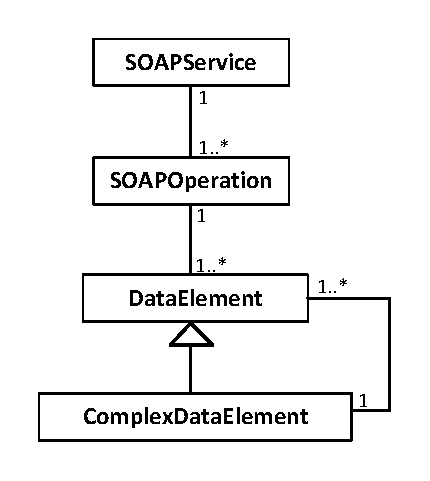
\includegraphics[scale=0.6]{images/wsdl-simplified}

\caption{Simple model for describing SOAP Services.}
\label{wsdl-Simplified}

\end{figure}

In the model above, \emph{DataElement} and \emph{ComplexDataElement} elements represent \emph{simple }and\emph{ complex types} (\emph{types})
respectively, which compose the message exchanged when invoking a service operation. Typically the terms used in defining such elements of the WSDL descriptor follow naming conventions commonly adopted by programmer, e.g. using \texttt{CamelCase} compound words for identifying operations, types and services. Similarly, sometimes documentation tags contain HTML encoded data. Therefore it is necessary to get the content into a proper format to enable further processing. This involves the use of text mining techniques such as \emph{tokenization},\emph{POS (Part-of-speech) tagging } and \emph{spell checking} whose description is addressed in section \ref{subsub:Service-documentation-cleaning}.

\subsubsection{XML-RPC and REST Services}
\label{subsubsec:rpc-rest}
As it was mentioned at the beginning of section \ref{subsec:analysis-ws-doc}, Web service documentation---except for SOAP services---doesn't meet
any standard format. XML-RPC and REST services, are commonly described by HTML pages, which provide information regarding service functionality and endpoints \footnote{For example: (XML-RPC) ,\href{http://www.benchmarkemail.com/API/Library}{http://www.benchmarkemail.com/API/Library} (REST) \href{https://dev.twitter.com/docs/api/1.1}{https://dev.twitter.com/docs/api/1.1}}. Usually the content of such pages doesn't follow a formal structure, making it difficult to extract relevant information in an automated way. There are some initiatives, including \emph{ProgrammableWeb} and
\emph{APIhub} \footnote{Available at: \href{http://www.apihub.com/}{http://www.apihub.com/}}, which promotes the creation of centralized API directories, where service documentation is uniformly stored, by following a regularstructure. However, a major issue regarding these initiatives is that documentation must be registered manually, so more often than not the information provided either contains errors (typos, broken links) or is outdated.

Given this limitation, it was decided to deal with documentation that developers provide on API websites. This way, we apply on each HTML page an analysis that involves identifying recurring patterns (which depends on the service type, either XML-RPC or REST) and document segmentation for extracting relevant information regarding service functionality. This analysis is supported on the approach of Ly et al. formulated in \cite{Ly:2012}.

\paragraph{Analysis of XML-RPC service documentation}
\label{parag:rpc}
Similar to SOAP services, an XML-RPC service defines a set of operations or procedures that clients can invoke remotely. The documentation of this kind of services, deals with the operations they expose, the arguments they require for their invocation, and usually specifies the service endpoint (URI) and the HTTP method used for communication.

The description of operations within the same XML-RPC service documentation tends to share similar structure and content. Thus, for example, operation identifiers are usually defined by terms in \texttt{CamelCase} notation, composed of a verb and a noun (e. g., \emph{getWeather}). Also, given that this kind of documentation is intended for humans, its content is articulated with recurrent visual clues that help identify operation description blocks within the HTML page: e.g., operation identifiers may be enclosed in \texttt{<h3>} tags and their natural language descriptions\emph{ }in \texttt{<p>} tags. Then, it is possible to use those local patterns present in each of the service documentation pages, for extracting the information blocks regarding service operations. 

Prior to the extraction of operation description blocks, a preprocessing step is required for getting rid of images, scripts, malformed tags and formatting tags (\texttt{<b>}, \texttt{<strong>}, \texttt{<i>}, etc.) from HTML documentation pages.

Then the operation description blocks are extracted, by following the steps below: 

\begin{enumerate}
 \item Extraction of \texttt{CamelCase} terms composed of a verb and a noun (which make up the set of candidate operations identifiers), while keeping track of the HTML tag that encloses them.
 \item Identify the most commonly used tag (\emph{elected tag}) for the operation identifiers found in the first step.
 \item Finally, out of all the operation identifiers found in step \#1, only retain identifiers within \emph{elected tags}. The page is then segmented according to the scope of the tags enclosing each of the chosen operation identifiers.
\end{enumerate}

By following the above procedure, it is possible to identify and extract the textual data from operation description blocks, such as that illustrated in Figure \ref{xml-rpc-op-block}.

\begin{figure}
 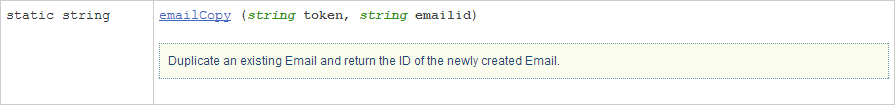
\includegraphics[scale=0.5]{images/xml-rpc-operation-block}

 \caption{Operation description block - XML-RPC service. {\scriptsize Source:
 \protect\href{http://www.benchmarkemail.com/API/Library}{http://www.benchmarkemail.com/API/Library}}}
 \label{xml-rpc-op-block}
\end{figure}

\paragraph{Analysis of REST APIs documentation}
\label{parag:rest}
REST services operate according to the principles and constraints addressed in section \ref{sub:REST-Architetural-Style}. While nowadays there is a seemingly increasing adoption of this architectural style for building web services, actually only a few of them support all the guidelines that REST defines. In terms of the Richardson's maturity model explained in section \ref{sub:REST-APIs}, most of the existing REST services are in fact \emph{level one }services\emph{ }(URI supported), while few of them qualify as \emph{level two }(URI \& HTTP supported) and \emph{level three} (RESTFul: URI, HTTP \& Hypermedia supported) services.

Documentation of this kind of services, provided as HTML pages, is focused on the concept of resources and the parameters used for identifying them, which are encoded into URI templates (e.g., \texttt{/\{resource\}/\{property\}/}). In addition, this documentation specifies the allowed HTTP methods
(\texttt{GET, POST, PUT, DELETE}, etcetera) for each of the resources hosted by the service. See for example the documentation available on the website of the twitter API for developers shown in Figure \ref{twitter-rest-api}.

\begin{figure}
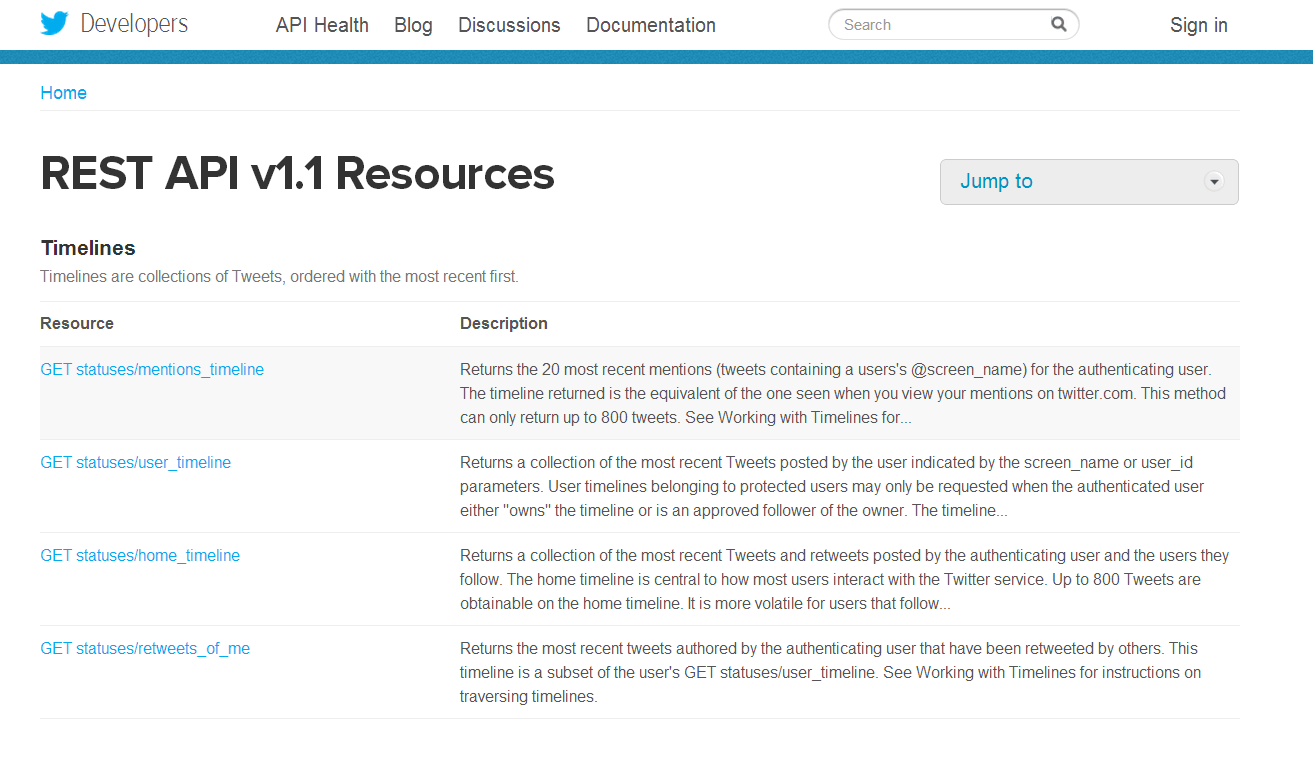
\includegraphics[scale=0.33]{images/twitter-rest-api}

\caption{Documentation of the Twitter REST API.{\scriptsize{} Source: \protect\href{https://dev.twitter.com/docs/api/1.1}{https://dev.twitter.com/docs/api/1.1}}}
\label{twitter-rest-api}

\end{figure}

This way, the analysis of REST services documentation focuses on detection and extraction of resources description blocks, which contain URI templates, HTTP methods and usually a description in natural language. Since REST API developers tend to adopt a recurring pattern for documenting
the service resources, it is possible to perform a segmentation procedure on the HTML content, in order to extract the mentioned description blocks. 

Such a procedure starts from the analysis of the HTML DOM tree to perform the steps listed below:

\begin{enumerate}
 \item Segment the HTML document into blocks containing URIs and HTTP methods. 
 \item Compute the similarity between the blocks found in step \#1, and retain those having the same structure.
 \item Extract the information of each resource, contained within the blocks identified in the previous step: resource URI, supported methods and description in natural language.
\end{enumerate}

For conducting the second step of the previous procedure, the authors of \cite{Ly:2012} rely on the concepts of \emph{entropy} and \emph{node internal structure}. Entropy is a measure that quantifies local patterns present in segments of the HTML document, so that a high entropy suggests
an irregular structure, while a low entropy denotes a substantial similarity. The internal structure of a node from the HTML DOM tree, consists in the concatenation of the tags that make up such node, so for example, given the following page segment \texttt{<div><a><span>link</span></a>\\<p>text</p></div>}, the internal structure of the \texttt{div} node is: \texttt{<div><a><span><p>}.

This way, the entropy measure estimates the similarity between the document segments found in step \#1, which is subsequently used for obtaining the set of resources descriptor blocks included in the service documentation.

\subsubsection{Service documentation pre-processing}
\label{subsub:Service-documentation-cleaning}
Often, the information that developers provide in service descriptors follows naming conventions commonly used in programming languages, in particular they use compound words such as \emph{helloword}, \emph{hello\_world} or \emph{helloWord} for identifying operations, resources and parameters. Also, it might be possible for descriptions in natural language to include content encoded into HTML or XML tags, which are used for formatting the text or providing structure to it. 

A requirement for further analyze the information extracted from service documentation (see end of section \ref{sec:motivation_background}) consists in processing such information and turning it into plain text, which involves splitting compound words and getting rid of HTML or XML tags. To this end it has been decided to use certain text mining techniques, including \emph{tokenization}, \emph{spell checking }and \emph{POS tagging}, whose description is addressed below. 

\paragraph{Tokenization}
\label{parag:tokenization}
This is a procedure that allows breaking a sequence of characters up into its composing tokens. The information extracted from service descriptors is subject to this process to generate the list of terms included within identifiers of operation, resources and types, as well as the text of descriptions in natural language. So, for example the list of tokens contained in the sequence ``\emph{getWeatherByCity}'' is: \{\textquotedblleft{}\emph{get}\textquotedblright{}, \textquotedblleft{}\emph{Weather}\textquotedblright{} \textquotedblleft{}\emph{By}\textquotedblright{}, \textquotedblleft{}\emph{City}\textquotedblright{}\}. In the previous example, the method for breaking the compound term up relies on detecting transition from lowercase to uppercase along the sequence. However, there are some cases where this procedure is not that straightforward: e.g., the sequence ``\emph{getweatherbycity}'' doesn't use letter case for telling tokens apart. In these special cases a spell checking technique is used, as 
outlined next.


\paragraph{Spell checking}
\label{parag:spell-checking}
It is clear for a human that strings \textquotedblleft{}\emph{homeaddress}\textquotedblright{} and \textquotedblleft{}\emph{home address}\textquotedblright{} contain the same information. However for machines those are two different sequences of characters and there is no trivial way for it to tell that they are equivalent strings. This turns out to be a common problem in Information Retrieval \cite{Airio:2006} known as \emph{compound splitting}. For tackling this compound splitting problem, we use a mechanism based on term look up over a tree-like data structure called \emph{Trie} \cite{Fredkin:1960} which in this particular case encodes the terms from the \emph{words }dictionary \footnote{Example available at: \href{http://www.cs.duke.edu/~ola/ap/linuxwords}{http://www.cs.duke.edu/$\sim$ola/ap/linuxwords}}, included in Unix-like operating systems. This data structure usually supports spell checking and autocomplete software, used in search engines and some other web and mobile applications.

\emph{Trie-based }search is similar to the way we look up words in a dictionary, i.e. by using prefixes. For extracting the terms that make up a compound word an iterative procedure is conducted: (1) It divides the sequence of characters into segments with different length; (2) it look up each of the segments in the Trie. This process continues until all the segments obtained in step \#1 match terms included in the dictionary. Table \ref{trie-example}, shows this procedure applied on the sequence \textquotedblleft{}\emph{homeaddress}\textquotedblright{}.

\begin{table}
\caption{Trie-based compound splitting for \textquotedblleft{}\emph{homeaddress}\textquotedblright{}.}


\center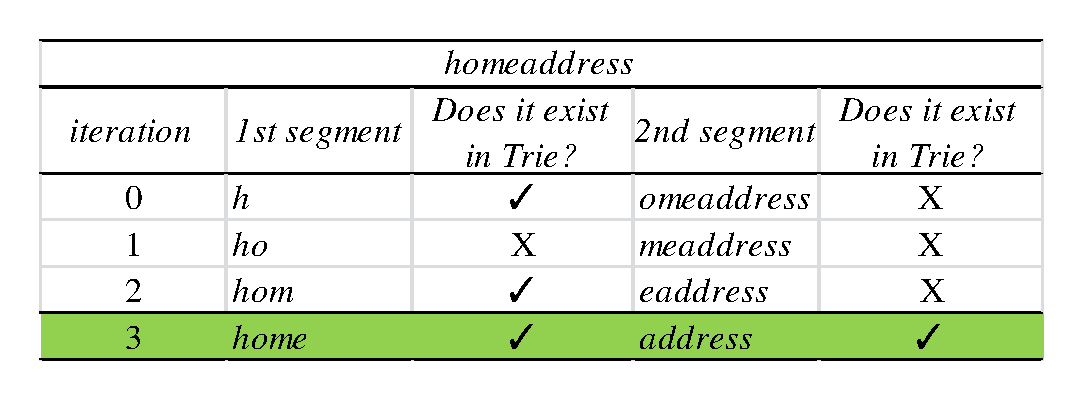
\includegraphics[scale=0.5]{images/example-trie-spellchecking-en}\label{trie-example}
\end{table}



\paragraph{Part-of-speech (POS) tagging}
\label{parag:part-of-speech}
This technique, is used for detecting candidate operations described in the documentation of XML-RPC services. According to the analysis outlined in section \ref{sub:Analysis-of-XML-RPC}, the operations hosted by this kind of services, are frequently identified by \texttt{CamelCase} terms joining at least a verb and a noun (e. g., \emph{getWeather}). POS tagging allows specifying the \emph{lexical category} (verb, noun, pronoun, adverb, etcetera) corresponding to each term in a text or sentence. This way it is possible to filter out the compound words included in XML-RPC service documentation and extracting the set of candidate operations. The POS tagging technique used in our case is the one conceived by Toutanova, outlined in \cite{Toutanova:2003} and developed inside The \emph{Stanford Natural Language Processing Group}.

By applying the techniques explained above on the documentation of Web services, the noise involved in the statistical analysis intended
to identify groups of similar services is reduced. As defined at the end of section \ref{sub:REST-APIs}, this analysis is the second of the key processes that comprise the approach documented herein. The description of this second process is addressed in the section below.